\chapter{Lyrics-based methods}\label{chap:lyrics_methods}
 In this chapter we will briefly describe some of the most prominent methods to represent songs based on their lyrics. After specifically focusing on the positive and negative aspects of these methods, we will select suitable candidates for testing and potentially for our web application. The reason to explore lyrics-based methods in this thesis is based on several factors. It is the belief of the authors that although the utilization of song lyrics is not completely unexplored as shown in Section \ref{sec:text_related_work}, there is space for innovative research. For example, to the best of our knowledge, there are no recommender systems that would rely solely on lyrics analysis. An advantage of these methods could lie in providing relevant recommendations that would be more variable compared other recommendations from other, more traditional techniques.

\section{Text embedding methods}
\subsection{Bag of Words}
The Bag of Words commonly referred to as BoW is a text representation method which counts how many times a word appears in a document. In the context of this thesis it counts how many times a word appears in the song lyrics.
BoW represents each text (song) as a word-count vector where each index corresponds to the number of times a certain word appeared in it. An advantage of this encoding is its simplicity. The simplicity, however, brings some drawbacks. It for example ignores the fact that some words which can be found in most documents have a smaller informative value than others that only appear in a small fraction of the documents. 

\subsection{TF-IDF}
Term Frequency-Inverse Document Frequency is another way of transforming documents into vectors. Unlike the BoW, Tf-idf does not measure only the counts of words in a document but it also measures their relevance. As can be deduced from the title term frequency, first the number of appearances of a word $t$ in each document $d$ proportional to the number of all words in that document - \textit{tf(t,d)} - is computed. Then comes the inverse document frequency part - \textit{idf} - where the words are weighted as seen in Formula \ref{eq:idf}. The words that appear frequently in most documents have lower weights than those who only appear in some.

\begin{equation}\label{eq:idf}
idf(t) = log\frac{1+n_d}{1+df(t)} + 1
\end{equation}

Formula \ref{eq:tf_idf} is then the final Tf-idf formula multiplying the word frequencies with their weights:

\begin{equation}\label{eq:tf_idf}
tf\textnormal{-}idf(t,d) = idf(t)*tf(t,d) 
\end{equation}
In both of the formulas above \textit{t} is the word \textit{d} is the document $ df(t) $ is the number of documents containing the word \textit{t} and \textit{n\textsubscript{d}} is the total number of documents. 

\subsection{Word2Vec}
Word2Vec is a two-layer neural network trained to encode the linguistic context of a word introduced by Tomas Mikolov \cite{DBLP:journals/corr/abs-1301-3781}. Each word has an assigned vector in a vector space of typically hundreds of dimensions generated from a large corpus. The position of a word corresponds to its context, meaning, that words that share common context are closer to each other.

There are two possible Word2Vec architectures, the continuous bag-of-words (CBOW) and the continuous skip gram. The CBOW predicts the current word from the words surrounding it --- the context. It does not keep the order of the surrounding context words. The skip gram does, which makes it slower but also more effective, especially for infrequent words \cite{DBLP:journals/corr/abs-1301-3781}. The Skip-Gram architecture takes one word and predicts all the context around it.
\begin{figure}[h]
    \centering
	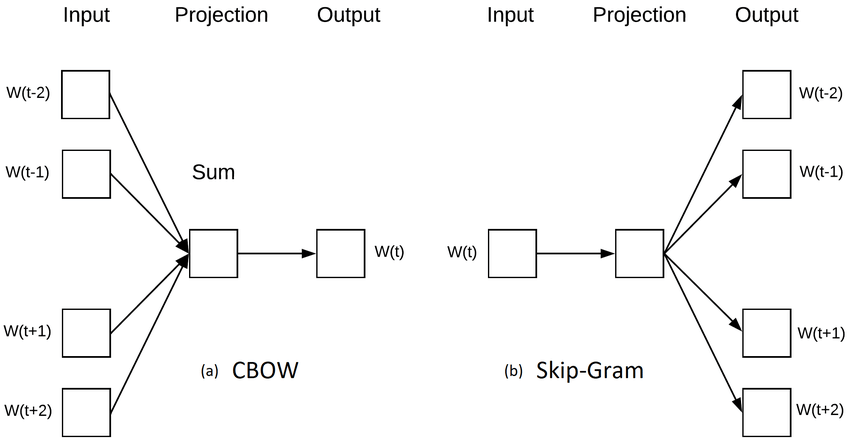
\includegraphics[height=70mm]{./img/cbow_skipgram_w2v_architecture.png}
	\caption{The CBOW and Skip-gram Word2Vec architectures from \cite{phdthesis}}
	\label{fig:cbow_skipgram_w2v_architecture}
\end{figure}


Multiple things have to be taken into account when training a W2V model. The information value of words that occur in all training documents is quite low so they can be removed to increase training speed. The dimensionality of the space also elevates accuracy only to a certain point so some threshold has to be set. Another parameter is the context window, which determines, how many words before and after a given word are included as its context.

\subsection{Doc2Vec}
Doc2Vec as is an unsupervised algorithm that learns the feature representation of texts with varying lengths and encodes them into vectors of the same length. As the name suggests it is heavily based on the idea of Word2Vec. It was also first presented by the same group of researches in this paper \cite{DBLP:journals/corr/LeM14}. The main idea of the method is to use the Word2Vec model but add one more vector to represent the paragraph as a whole. As in the Word2Vec model, there are two architectures for the Doc2Vec approach. The Distributed Memory (DM) version of Paragraph vector and the Distributed Bag of Words (DBOW) version of the Paragraph vector. The DBOW is faster but does not consider the order of the words as it predicts a random group of words from the paragraph vector. The DM on the other hand takes previous words and the paragraph vector into account and predicts just one word. This way, because the paragraph does not shift across the text, the DM architecture is able to capture some word order but it requires more time to be trained.
\begin{figure}[h]
    \centering
	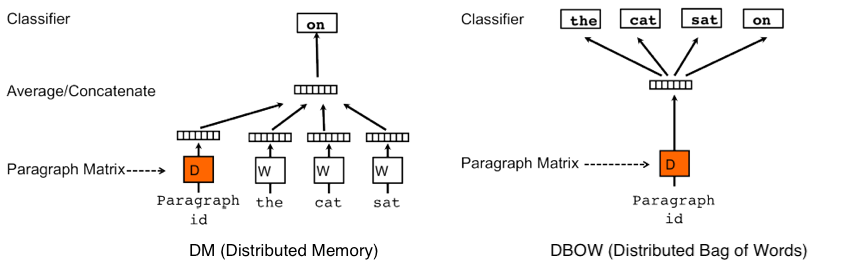
\includegraphics[width=140mm]{./img/DV_DBOW_doc2vec_architectures.png}
	\caption{The Doc2Vec DM and DBOW architecture taken from \cite{DBLP:journals/corr/LeM14}}
	\label{fig:dbow_dm_d2v_architecture}
\end{figure}
\subsection{Self organizing maps}
A self organizing map (SOM) is a type of a neural network that learns how to reduce the dimension of input data in an unsupervised manner. SOMs were introduced by Teuvo Kohonen \cite{Kohonen1982}. They use competitive dimensionality reduction (meaning the nodes in the SOM network compete to get the right to respond to the input data) which is quite unusual for neural networks as they usually use backpropagation. The models that SOMs compute are (usually) two dimensional spaces of neurons (called \textit{codebook} vectors) where similar examples are close to each other and dissimilar examples further from each other.

The SOM network is trained through an iterative process which is visualized in Figure \ref{fig:som_training}. It chooses one sample \textbf{x} \( \in R^n \) from the input training set at random and teaches it to itself. During teaching, the network feeds the chosen sample into all its units. A winner unit is calculated based on a similarity measure (usually Euclidean distance) between \textbf{x} and the \textit{codebook} vectors. Finally the values of the network units are updated. The best-matching unit is moved a closer to \textbf{x} and so are all the topological neighbours of the best unit.

The neighbours are defined by a neighbourhood function. It decreases with time and decides how radical the change around the winner will be. There are multiple functions that can be used. One can use the Gaussian kernel around the winner, however this is quite computationally expensive. A good and more efficient function is sometimes called the \textit{"bubble"} function which is constant over the whole neighbourhood of the winner and zero elsewhere \cite{SOM_training}.

\begin{figure}[H]
\begin{minipage}{\textwidth}
    \centering
	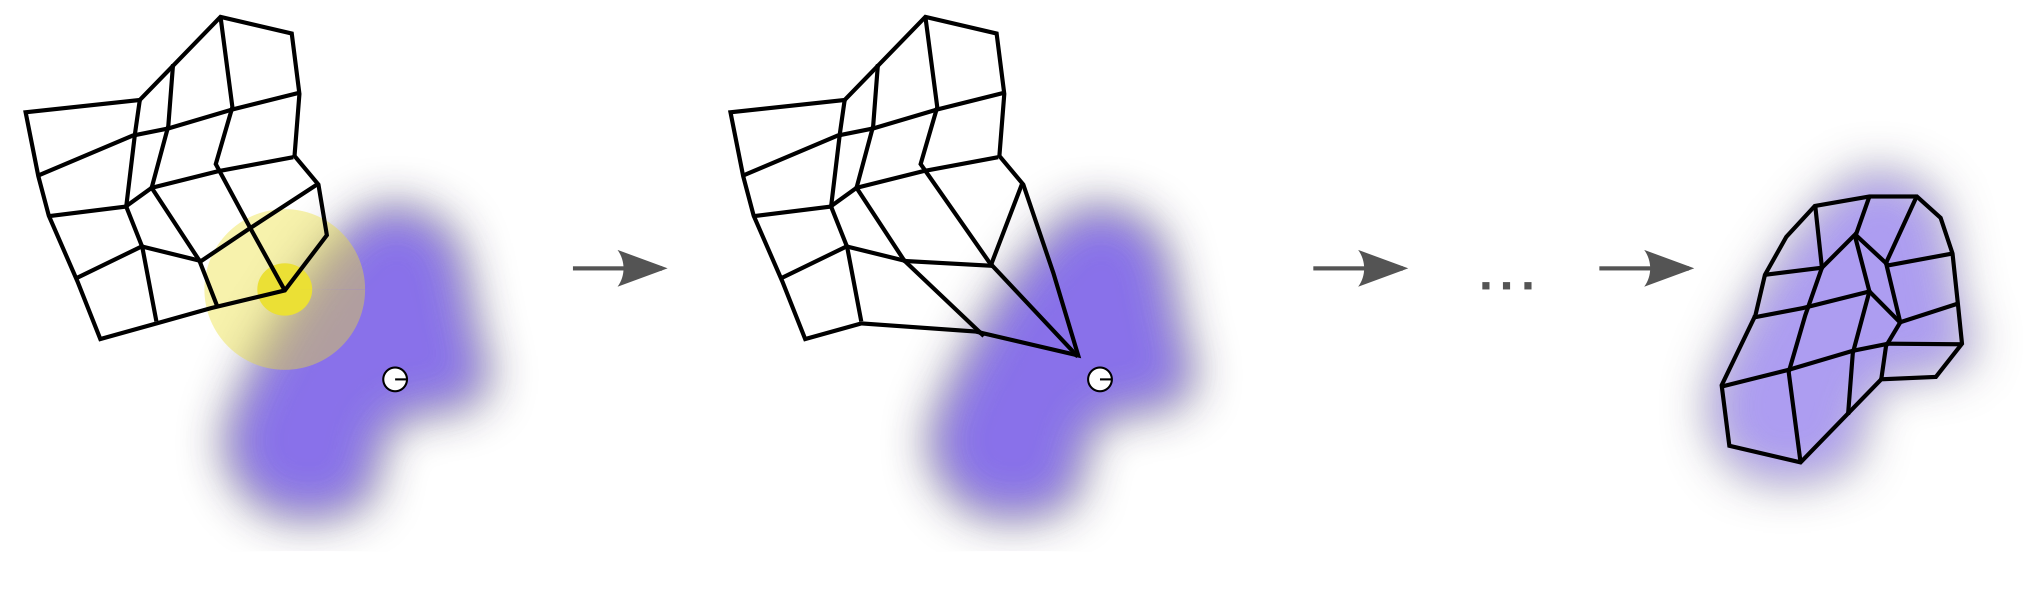
\includegraphics[width=140mm]{./img/Somtraining.png}
	\caption[A visualization of the training used for SOM networks]{Visualization of the training algorithm used for SOM networks. The blue area represents the distribution of the data. The white dot is the randomly selected sample. On the left, the SOM network nodes are randomly spread accross the space. When finding a winner (middle) and its defined neighbourhood (the yellow area) the network moves towards the datapoint and eventually after repeated iterations spreads mimicking the distribution of the data (left). This image is taken from Wikipedia\footnotemark}
	\label{fig:som_training}
\end{minipage}
\end{figure}

\footnotetext{https://commons.wikimedia.org/wiki/File:Somtraining.svg}

\section{Related work}\label{sec:text_related_work}

 There are several papers on music recommendation based on lyrics. For example \cite{Gossi2016LyricBasedMR} has shown, that simple Tf-idf song embedding was 12.6 times more accurate then just random suggestions on the musiXmatch dataset\footnote{https://labrosa.ee.columbia.edu/millionsong/musixmatch}.  In \cite{inproceedings} the authors compared the Doc2Vec and the SOM algorithm using cosine similarity for vector aggregation on a dataset containing Hindi songs and found that in their experiments, the SOM outperforms Doc2Vec. Paper \cite{DBLP:journals/corr/Tsaptsinos17} even studies using intact lyrics as input for Recurrent (LSTM) and Hierarchical neural networks and evaluates it based on genre classification.

\section{Text representation choices}
When choosing methods for our web application there are several factors to consider. Besides the expected accuracy of the algorithms, which is often difficult to guess since lyrics-based recommendation methods have not been researched extensively, we have to consider the implementation as well as temporal complexity features of all the methods. Also, the fact that we want to focus more on a cross-sectional approach rather than a thorough optimization of one particular algorithm, means we prefer diversity in our chosen algorithms.  \\

The Bag of Words representation could be a good choice to get some kind of baseline results. Nevertheless, since the Tf-idf algorithm is widely based on the BOW and is still quite simple, we choose \textbf{Tf-idf} as our baseline. As mentioned at the beginning of this chapter, it was shown to be 12.6 times more accurate on the musiXmatch Dataset (MXD)\footnote{https://labrosa.ee.columbia.edu/millionsong/musixmatch} than just random suggestions, and that is what we hope to achieve with all of our text methods. A downside of the Tf-idf method is the length of its vectors. Even though they consist mostly of zeros, for our dataset, the length of each of them is over 40,000. 

Word2Vec and Doc2Vec are two similar approaches. The issue with Word2Vec when representing a whole document, in our case the lyrics for one song, is the transition between the word vectors and the whole document encoding. A commonly used aggregation method is to define the document vector as the mean of all the word vectors. 

Doc2Vec does not suffer from this problem, as its default is suited to represent a complete text. However, the problem with Doc2Vec is the amount of data it needs for training. Because every document is one sample, the number of documents necessary to achieve reasonable results is much higher than for Word2Vec where one sample is one word. What is also convenient with Word2Vec is, that there already exists a pre-trained Word2Vec model from Google\footnote{https://code.google.com/archive/p/word2vec/}. It consists of 3 million words with a 300-dimensional vector for each. Three hundred dimensions is a reasonable number (especially considering the fact that the Tf-idf vectors have over 40,000 dimensions). It was trained on roughly a billion words from a Google News dataset. Therefore we chose the Word2Vec model over the Doc2Vec.  

The choice of \textbf{Word2Vec} was also justified by the lack of recommendation algorithms based on it. We also decided to implement the \textbf{SOM} network rather than Doc2Vec to represent songs based on a study showing, that Self organizing maps perform better than a Doc2Vec-based algorithm \cite{inproceedings}. It also does not need as much data as the Doc2Vec to be trained. 

One more thing we had to chose for the SOM was the form of the input. We decided to try the W2V representation. Mainly because the training of a self organizing map is quite computationally expensive and having vectors with over 40,000 dimensions would make it extremely time-consuming. We did not give up on the Tf-idf representation though. We trained another SOM where used Tf-idf vectors pre-processed by PCA which were reduced to length 4,457. 

